\documentclass[12pt,a4paper,parskip=full]{scrartcl}

\usepackage{bbding}
\usepackage{pifont}
\usepackage{wasysym}
\usepackage[margin=1in]{geometry}
\geometry{a4paper}
\usepackage{xcolor}
\definecolor{red}{HTML}{cc0000}
\definecolor{gray}{HTML}{666666}
\usepackage{sectsty}
\sectionfont{\color{red}}
\subsectionfont{\color{red}}
\subsubsectionfont{\color{red}}
\usepackage{graphicx}
\usepackage{hyperref}
\usepackage{amssymb}
\usepackage[style=footnote-dw]{biblatex}
\bibliography{S@SGuideBib}
\setlength\bibitemsep{0.5\baselineskip}

\usepackage{enumitem}
\setitemize{noitemsep}
% \setlist{noitemsep, topsep=-5pt}
% \setlength\itemsep{-0.10em}

\renewcommand{\labelitemi}{$\cdot$}
\renewcommand{\labelitemii}{$\cdot$}
\makeatletter
\let\latexl@section\l@section
\def\l@section#1#2{\begingroup\let\numberline\@gobble\latexl@section{#1}{#2}\endgroup}
\makeatother

\usepackage[T1]{fontenc}
\fontfamily{verdana}

\usepackage{scrlayer-scrpage}{}
\makeatletter
\renewcommand{\@seccntformat}[1]{}
\makeatother

\setlength\parindent{0pt}{}

\title{\Huge{\color{red}\textbf{The Scrum@Scale 
\textsuperscript{\copyright} 
Guide}}}
\subtitle{\color{gray}Ostateczny Przewodnik po Scrum@Scale:\\ Skalowanie, które działa}
\author{Krystian Kaczor}
\date{20190601}

\begin{document}

%\tableofcontents
%\newpage

\section{Cel Przewodnika Scrum@Scale}

Scrum, jak to zostało nakreślone w Przewodniku po Scrumie, jest frameworkiem do rozwijania, dostarczania i utrzymywania złożonych produktów przez pojedynczy zespół. Od jego powstania, jego wykorzystanie rozszerzyło się do tworzenia produktów, procesów, usług i systemów wymagających wysiłku wielu zespołów. Scrum@Scale został stworzony, żeby efektywnie koordynować ten nowy ekosystem zespołów w sposób, który optymalizuje ogólną strategię organizacji. Osiąga ten cel poprzez ustanowienie "minimalnej użytecznej biurokracji" przez bezskalową architekturę, która naturalnie rozszerza sposób w jaki pojedynczy Zespół Scrumowy działa na całą organizację.

Ten przewodnik zawiera definicje komponentów, które tworzą framework Scrum@Scale, włączając skalowane role, skalowane wydarzenia i artefakty przedsiębiorstwa, jak również zasady, które łączą je razem.

Dr. Jeff Sutherland zbudował Scrum@Scale w oparciu o fundamentalne zasady stojące za Scrumem, teorię Złożonych Systemów Adaptacyjnych, teorią gier i technologią zorientowaną obiektowo. Ten przewodnik został zbudowany z wkładem wielu doświadczonych praktyków Scruma w oparciu o rezultaty ich pracy w praktyce. Celem tego przewodnika jest, żeby czytelnik był w stanie samodzielnie zaimplementować Scrum@Scale.

\subsection{Dlaczego Scrum@Scale?}

Scrum został zaprojektowany dla pojedynczego zespołu, żeby mógł pracować w jego optymalnych możliwościach równocześnie zachowując utrzymywalne tempo. W praktyce, okazało się, że gdy liczba Zespołów Scrumowych w organizacji rosła, wydajność (działający produkt) i prędkość tych zespołów zaczęła spadać ze względu na problemy takie, jak zależności międzyzespołowe i duplikowanie pracy. Stało się oczywiste, że potrzebny był framework do efektywnej koordynacji tych zespołów, żeby osiągnąć linową skalowalność. Scrum@Scale jest zaprojektowany, żeby osiągnąć ten cel przez bezskalową architekturę.

Bezskalową architekturę można powszechnie znaleźć w systemach biologicznych takich jak ludzkie ciało, czy w projektowaniu procesorów, które wymaga umieszczenia miliardów tranzystorów w procesorze. Internet jest zaprojektowany, żeby być bezskalowym w ten sposób, że każdy węzeł ma tą samą strukturę co inny węzeł. Dzięki wykorzystaniu bezskalowej architektury organizacja nie jest ograniczona we wzroście w określonym kierunku przez zestaw arbitralnych zasad; raczej może organicznie rosnąć w oparciu o jej unikalne potrzeby i w utrzymywalnym tempie zmiany, które może być zaakceptowane przez grupy osób tworzących organizację. Prostota modelu Scrum@Scale model jest niezbędna dla  bezskalowej architektury i ostrożnie unika wprowadzania dodatkowej złożoności, która spowoduje spadek wydajności per zespół w miarę jak tworzone jest więcej zespołów.

Scrum@Scale jest zaprojektowany do skalowania poprzez organizację jako całość: wszystkie działy, produkty i usługi. Może być zastosowana w wielu dziedzinach we wszystkich typach organizacji w przemyśle, rządzie czy środowiskach akademickich.

\subsection{Definicja Scrum@Scale}

\textbf{Scrum}: Framework w ramach, którego ludzie mogą rozwiązywać złożone adaptacyjne problemy, produktywnie i kreatywnie dostarczając użyteczne produkty o możliwie największej wartości.

Przewodnik po Scrumie jest minimalnym zestawem funkcjonalności, który pozwala na inspekcję i adaptację poprzez radykalną transparencję, żeby prowadzić do innowacji, zadowolenia klienta, wydajności i zasdowolenia zespołu.

\textbf{Scrum@Scale}: Framework w ramach, którego sieci Zespołów Scrumowych działające zgodnie z Przewodnikiem po Scrumie mogą rozwiązywać złożone adaptacyjne problemy, kreatywnie dostarczając  produkty o możliwie największej wartości.

\textbf{UWAGA}: Te "produkty" mogą być sprzętem, oprogramowaniem, złożonymi zintegrowanymi systemami, procesami, usługami, itd. w zależności od dziedziny Zespołów Scrumowych.

Scrum@Scale jest:
\begin{itemize}
	\item Lekki - minimalna użyteczna biurokracja
	\item Prosty do zrozumienia - składa się jedynie z Zespołów Scrumowych
	\item Trudny w praktyce - wymaga zaimplementowania nowego modelu operacyjnego
\end{itemize}

Scrum@Scale jest frameworkiem do skalowania Scruma. Radykalnie upraszcza skalowanie poprzez wykorzystanie Scruma do skalowania Scruma.

W Scrumie, zatroszczono się o to, żeby rozdzielić odpowiedzialność za "Co" od "Jak". Z taką samą troską w Scrum@Scale dba się, żeby jurysdykcja i odpowiedzialność były wyraźnie zrozumiane w celu eliminacji bezproduktywnego konfliktu organizacyjnego, który powstrzymuje zespoły od osiągnięcia ich optymalnej produktywności.

Scrum@Scale składa się z komponentów, które pozwalają organizacji dopasować jej strategię transformacji i implementacji. To daje jej możliwość celować w jej przyrostowo priorytetyzowane wysiłki zmian w obszar(y), które uważa za najbardziej wartościowe albo najbardziej potrzebujące zmiany, a następnie zrobić postępy w innych.

W ramach rozdzielenia jurysdykcji, Scrum@Scale zawiera dwa cykle: Cykl Scrum Mastera ("Jak") i Cykl Product Ownera ("Co"), stykające się w dwóch punktach. Te kręgi wzięte razem dostarczają potężny framework do koordynacji wysiłków wielu zespołów wzdłuż pojedynczej ścieżki.

\subsection{Kultura Oparta Na Wartościach}

Poza rozdzieleniem odpowiedzialności za "Co" i "Jak", dalszym celem Scrum@Scale jest zbudowanie zdrowych organizacji poprzez stworzenie kultury opartej na wartościach w empirycznym otoczeniu. Wartościami Scruma są: Otwartość, Odwaga, Skupienie, Szacunek, and Zaangażowanie. Te wartości kierują empirycznym podejmowaniem decyzji, które polegają na trzech filarach przejrzystości, inspekcji i adaptacji.

Otwartość wspiera przejrzystość całej pracy i procesów, bez której nie ma możliwości uczciwego sprawdzenia ich i próby dostosowania ich ku lepszemu. Odwaga dotyczy podejmowania śmiałych kroków wymaganych do dostarczenia wartości szybciej na innowacyjne sposoby.

Skupienie i Zaangażowanie odnoszą się do sposobu w jaki traktujemy nasze obowiązki wynikające z pracy, nadając najwyższy priorytet dostarczaniu wartości klientowi. Ostatecznie, to wszystko musi wydarzyć się w środowisku opartym o szacunek dla osób wykonujących pracę, bez których nic nie może być stworzone.

Scrum@Scale pomaga organizacjom prosperować poprzez wspieranie modelu przywództwa transformacyjnego, które sprzyja pozytywnemu środowisku do pracy w utrzymywalnym tempie i stawia zaangażowanie do dostarczenia wartości z punktu widzenia klienta na czele naszych wysiłków.

\subsection{Komponenty Scrum@Scale\textregistered ~Framework}

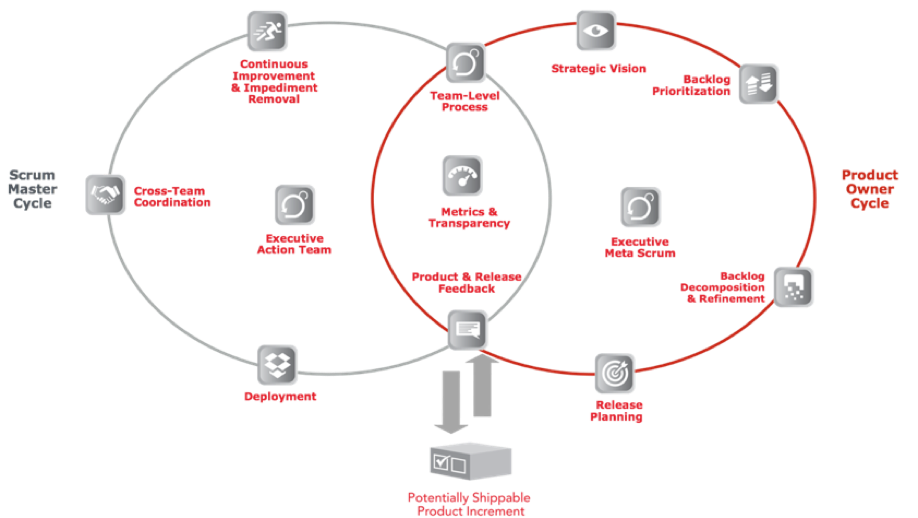
\includegraphics[width=1.0\linewidth]{SMPO-Cycle.png}

\section{Skalowana Struktura: Scrum of Scrums}

Zbiór Zespołów Scrumowych, które potrzebują skoordynować się, żeby dostarczyć wartość do klientów tworzy \textbf{Scrum of Scrums (SoS)}. Ten zespół jest odpowiedzialny za w pełni zintegrowany zbiór potencjalnie nadających się do wydania przyrostów produktu na koniec każdego Sprintu ze wszystkich uczestniczących zespołów. SoS działa jak Release Team i musi być w stanie dostarczyć wartość wprost do klientów.

Scrum of Scrums jest a Zespołem Scrumowym z normalnymi rolami Scrum, wydarzeniami i artefaktami spójnymi z Przewodnikiem po Scrumie. Jednakże, biorąc pod uwagę skalowaną naturę SoS są pewne dodatkowe rzeczy do wzięcia pod uwagę.

\subsection{Role SoS}

SoS potrzebuje mieć wszystkie umiejętności potrzebne do dostarczenia w pełni zintegrowanego, potencjalnie nadającego się do wydania Przyrostu Produktu na koniec każdego Sprintu i umożliwić koordynację pomiędzy zespołami kiedy jest to konieczne. Może to wymagać doświadczonych architektów, liderów QA, członków Zespołu Własności Produktu, i wachlarzu innych umiejętności operacyjnych.

\subsubsection{Product Owner Team}

Grupa Właścicieli Produktu, która koordynuje wspólny backlog zasilający sieć zespołów jest Zespołem Scrumowym zwanym \textbf{Product Owner Team}. Dla każdego SoS jest jest przypisany Product Owner Team, który uzgadnia priorytety zespołów wzdłuż pojedynczej ścieżki, żeby one skoordynowały swoje backlogi zespołu i zbudować uzgodnienie z interesariuszami, żeby wspierać backlog.

Product Owner zespołu jest odpowiedzialny za tworzenie i priorytetyzowanie backlogu zespołu i może wciągać elementy backlogu ze wspólnego backlogu SoS do backlogu zespołu albo tworzyć niezależne elementy backlogu według własnego uznania.

Głównymi zadaniami Product Owner Team są:

\begin{itemize}
	\item stworzyć nadrzędną wizję produktu i zapewnić, że jest widoczna w organizacji.
	\item stworzyć uzgodnienie z interesariuszami, żeby zapewnić implementację backlogu.
	\item stworzyć jeden, spriorytetyzowany backlog, zapewniajac, że unikane jest powielanie pracy.
	\item zapewnić, że przeszkody i dług techniczny są odpowiednio spriorytetyzowane w backlogu.
	\item stworzyć minimalną, jednolitą "Definicję Ukończenia", która dotyczy wszystkich zespołów.
	\item rozwiązywać zależności wskazane przez zespoły.
	\item stworzyć skoordynowany Plan Wydań i prognozę poza aktualny Plan wydań (często zwane roadmapą).
	\item zdecydować jakie metryki dają wgląd w produkt i rynek i je monitorować.
\end{itemize}

Zespoły Product Owner Team, tak jak SoSy działają na własną rękę jak Zespoły Scrumowe. Jako takie, muszą mieć kogoś, kto działa jak Scrum Master i utrzymuje skupienie podczas dyskusji. Potrzebują też pojedynczej osoby, która jest odpowiedzialna za koordynowanie powstawania pojedynczego Product Backlogu dla wszystkich zespołów w ramach Scrum of Scrums. Ta osoba jest określona jako \textbf{Chief Product Owner}.

\subsubsection{Chief Product Owner (CPO)}

\textbf{Chief Product Owner} (CPO) koordynuje priorytety pomiędzy Product Ownerami, którzy pracują z konkretnymi zespołami. Uzgadniają priorytety zgodnie z potrzebami Interesariuszy i Klientów. Może to być PO konkretnego zespołu pełniący tą rolę albo osoba konkretnie dedykowana do tej roli. Odpowiedzialność CPO jest taka sama jak PO zespołu, ale w skali CPO jest odpowiedzialny za:

\begin{itemize}
	\item stworzyć strategiczna wizję dla całego SoS.
	\item stworzyć pojedynczy, spriorytetyzowany backlog wartości do dostarczenia przez wszystkie zespoły.
	\begin{itemize}
		\item Uwaga: te elementy są zazwyczaj większymi Elementami Backlogu Produktu, które będą potrzebowały dalszej pielęgnacji i dekompozycji przez PO zespołów.
	\end{itemize}
	\item pracować blisko z powiązanym Scrum of Scrums Masterem (zdefiniowane poniżej), tak, żeby Plan Wydań stworzony prze zespół Product Ownera mógł być efektywnie wdrożony.
	\item monitorować feedback klientów produktu, a także feedback na temat produktu z SoS i odpowiednie dostosowanie backlogu.
	\item na poziomie executive/meta, prowadzić MetaScrum, gdzie nadrzędny Product Backlog jest prezentowany i uzgodniony z interesariuszami.
\end{itemize}



\subsubsection{Scrum of Scrums Master (SoSM)}

Scrum Master Scrum of Scrums jest nazwany \textbf{Scrum of Scrums Master (SoSM)}. SoSM jest odpowiedzialny za wydanie połączonego wysiłku zespołów i musi:

\begin{itemize}
	\item uwidocznić postęp.  %make visible - uwidocznić
	\item uwidocznić dla organizacji backlog przeszkód.
	\item usuwać przeszkody, których zespoły nie mogą rozwiązać samodzielnie.
	\item facylitować priorytetyzację przeszkód, ze szczególną uwagą na zależności międzyzespołowe i rozdział backlogu.
	\item poprawić efektywność Scrum of Scrums.
	\item pracować blisko z Product Owner Team, żeby wdrożyć potencjalnie nadający się do wydania Przyrost Produktu przynajmniej raz w każdym Sprincie.
	\item skoordynować wdrożenie zespołu z Planem Wydań Product Ownera.
\end{itemize}

\subsection{Wydarzenia SoS}

\subsubsection{Postępowanie z Przeszkodami na poziomie SoS}

SoSM powinien sfacylitować wydarzenie Pielęgnacji Backlogu gdzie przeszkody są określone jako "gotowe" do usunięcia i zespół określa jak najlepiej usunąć je i po czym poznają, że są "ukończone". Elementy dotyczące usuwania przeszkód są priorytetyzowane dla zespołów w tym samym backlogu, który tworzy SoS CPO i Product Owner Team.

Szczególną uwagę należy zwrócić na Retrospekcją SoS, na której reprezentanci zespołów dzielą się tym, czego się nauczyli albo ulepszeniami procesu, które powiodły się w ich poszczególnych zespołach, w celu dzielenia się najlepszymi praktykami pomiędzy zespołami w ramach SoS.  %individual team - poszczególny zespół

\subsubsection{Scaled Daily Scrum (SDS)}

Ponieważ SoS musi na bieżąco odpowiadać na przeszkody zgłaszane przez uczestniczące w nim zespoły, przynajmniej jeden przedstawiciel (zwykle Scrum Master zespołu) każdego z uczestniczących zespołów musi uczestniczyć w \textbf{Scaled Daily Scrum (SDS)}. Wydarzenie SDS odzwierciedla Daily Scrum w sensie optymalizacji współpracy i wydajności sieci zespołów. Dowolna osoba lub liczba osób z uczestniczących zespołów może uczestniczyć w miarę potrzeb. Dodatkowo SDS:

\begin{itemize}
	\item jest ograniczony czasowo do maksymalnie 15 minut.
	\item musi być uczęszczany przez reprezentantów z każdego zespołu z Product Owner Team włącznie.
	\item jest forum gdzie reprezentacji zespołów dyskutują o tym co idzie dobrze, co jest ukończone i jak zespoły mogą pracować bardziej efektywnie. 
\end{itemize}
	
Kilka przykładów, co może być omawiane:
\begin{itemize}
	\item Jakie przeszkody stoją na drodze mojego zespołu do osiągnięcia ich Celu Sprintu (albo wpływające na najbliższe wydanie)?
	\item Czy mój zespół robi coś, co przeszkodzi innemu zespołowi w osiągnięciu ich Celu Sprintu (albo wpływają na najbliższe wydanie)?
	\item Czy odkryliśmy nowe zależności pomiędzy zespołami albo odkryliśmy istniejące zależności?
	\item Jakie odkryliśmy przeszkody, które mogą wpływać na wszystkie zespoły?
\end{itemize}

\section{Executive/Meta Level}

\subsection{Executive Action Team (EAT)}

Rola Scrum Mastera, która jest częścią Scrum of Scrums z punktu widzenia całej zwinnej organizacji jest nazwana \textbf{Executive Action Team (EAT)}. Zespół liderów tworzy zwinną bańkę w organizacji, której Model Referencyjny działa z własnymi zasadami, procedurami, który efektywnie integruje się z dowolną częścią organizacji, która nie jest zwinna. Jest właścicielem zwinnego ekosystemu, implementuje wartości Scruma i zapewnia, ze role Scrum są stworzone i wspierane.
%SoS's??
EAT jest ostatnim przystankiem dla przeszkód, które nie mogą być usunięte przez SoSy, które je zgłosiły. Dlatego, żeby je usuwać, EAT musi składać się z osób, które mają umocowanie polityczne i finansowe, żeby je usuwać. Funkcją EAT jest skoordynowanie wielu SoSów i zbudowanie interfejsu z nie-zwinnymi częściami organizacji.Tak jak w przypadku każdego zespołu, potrzebuje PO i SM, oraz żeby spotykać się codziennie. Muszą mieć również przejrzysty backlog.

Przykładowy diagram pokazujący EAT koordynujący 5 grup of 25 zespołów:

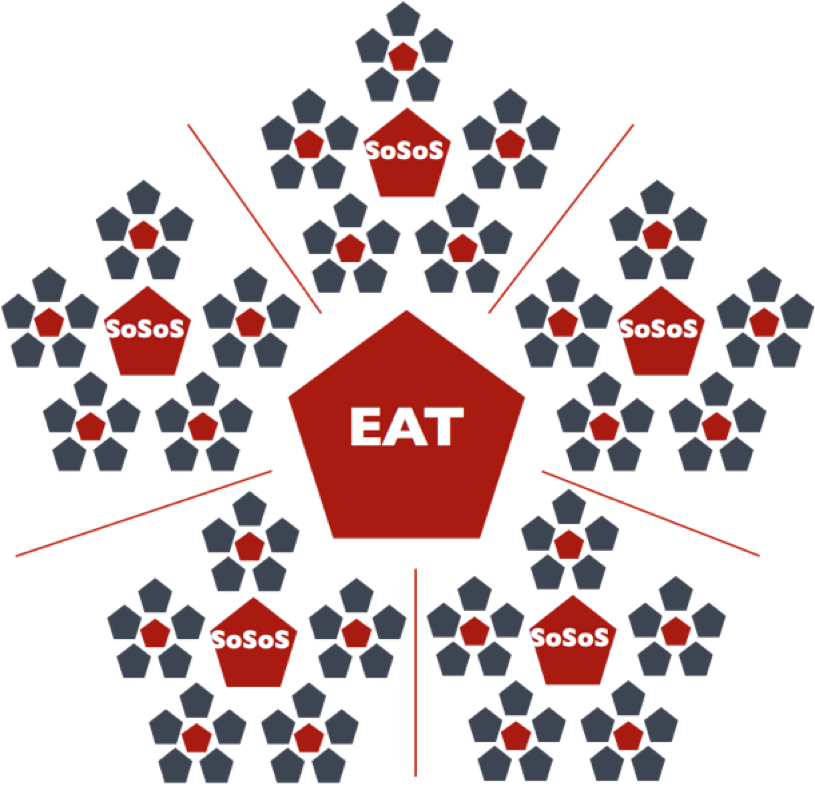
\includegraphics[width=\textwidth,height=\textheight,keepaspectratio]{SoS-EAT.png}

\subsubsection{Backlog i Odpowiedzialność EAT}

Scrum jest zwinnym systemem operacyjnym, który rożni się od tradycyjnego zarządzania projektami. Cała organizacja SM raportuje to EAT, który jest odpowiedzialny za wprowadzenie w życie tego zwinnego modelu operacyjnego przez ustanowienie, utrzymanie i wzmacnianie implementacji w organizacji.

Rolą EAT jest stworzyć Backlog Transformacji Organizacji (spriorytetyzowana lista zwinnych inicjatyw, zrealizowane) i zobaczyć jak to się odbywa. Na przykład, jeżeli istnieje tradycyjny Cykl Rozwoju Produktu w starej organizacji, nowy - zwinny Cykl Rozwoju Produktu, musi być stworzony, zaimplementowany i wspierany . Zwykle on lepiej wspiera zagadnienia jakości i zgodności niż stara metoda, ale zaimplementowana w inny sposób z innymi zasadami i wytycznymi. EAT zapewnia, że organizacja Product Ownerów jest stworzona i finansowana oraz, że ta organizacja jest reprezentowana w EAT, żeby wspierać te wysiłki.

EAT jest odpowiedzialny za jakość Scruma w organizacji. Jego odpowiedzialności obejmują, ale nie są odgraniczone do:

\begin{itemize}
	\item stworzenie zwinnego systemu operacyjnego dla Modelu referencyjnego w miarę jak skaluje się przez organizację, włączając w to zasady działania operacyjnego organizacji, procedury i wytyczne, żeby umożliwić zwinność.
	\item mierzenie i ulepszanie jakości Scruma w organizacji.
	\item zbudowanie zdolności do zwinności biznesowej w ramach organizacji.
	\item stworzenie centrum dla ciągłego uczenia się profesjonalistów Scruma.
	\item wspieranie poszukiwania nowych sposobów wykonywania pracy.
\end{itemize}

\subsection{Executive MetaScrum (EMS)}

Zespoły Product Owner Team umożliwiają projektowanie sieci Product Ownerów, która jest nieskończenie skalowalna razem z ich powiązanymi SoSami. Product Owner Team dla całej organizacji spotyka się z kluczowymi interesariuszami jako \textbf{Executive MetaScrum}. Do EMS należy wizja organizacji i on ustala strategiczne priorytety orientując zespoły wokół wspólnych celów.
%align?? orientować?
Przykładowy diagram pokazujący EMS koordynujący 5 grup 25 zespołów:

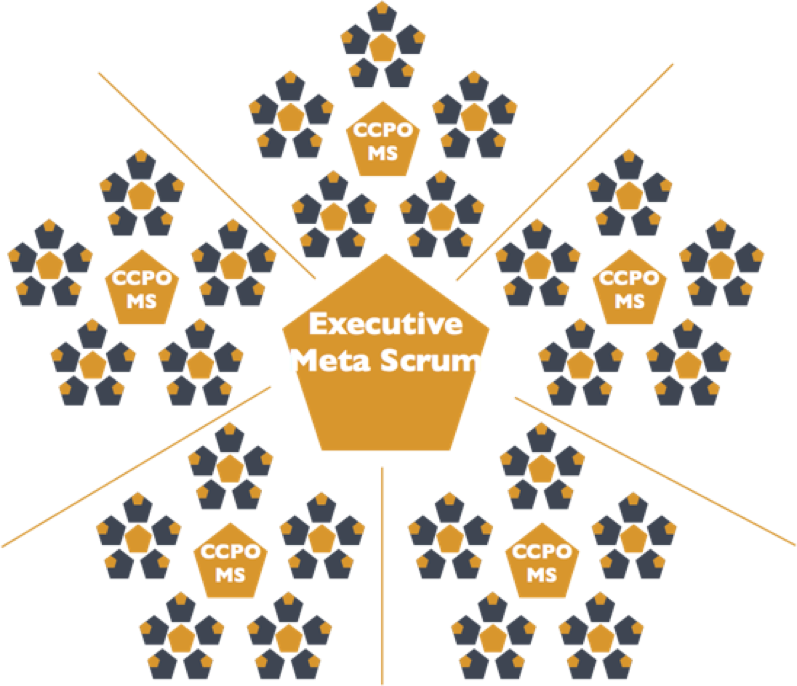
\includegraphics[width=1.0\linewidth]{ExecMetaScrum.png}

Executive MetaScrum Team przeprowadza spotkanie uzgadniające z interesariuszami, \textbf{MetaScrum Event}, w regularny rytmie przynajmniej raz na Sprint.

\begin{itemize}
	\item Członkowie Executive MetaScrum Team (albo proxy) uczestniczą w Wydarzeniu MetaScrum, gdzie Chief Product Owner prezentuje backlog produktu właścicielom biznesowym, którzy kontrolują finansowanie, personel, zobowiązania w stosunku do klientów. Wyrażają oni zmiany potrzebne w strategii, finansowaniu, przydzielaniu zasobów oraz wdrożeniach i współpracują z Chief Product Ownerami, żeby zbudować uzgodnioniony Backlog Produktu, który będą wspierać do następnego wydarzenia MetaScrum.
	\item To wydarzenie jest forum dla  liderów, interesariuszy, i właścicieli biznesowych do wyrażania ich preferencji lub czasem pilnych żądań, które mogą spowodować, że backlog Chief Product Ownera zostanie zmieniony.
\end{itemize}

\section{Skalowanie}

\subsection{Skalowanie SoS}

W zależności od rozmiaru organizacji więcej niż jeden SoS może być potrzebny do dostarczenia bardzo złożonego produktu. W takich przypadkach z wielu  Scrums of Scrums może zostać utworzony \textbf{Scrum of Scrum of Scrums (SoSoS)}. SoSoS jest organicznym wzorcem Zespołów Scrumowych, który można skalować w nieskończoność. Każdy SoSoS powinien mieć SoSoSM i skalowane wersje każdego artefaktu i wydarzenia.

Skalowanie SoS redukuje liczbę ścieżek komunikacyjnych w ramach organizacji, także złożoność jest ograniczona. SoSoS styka się z SoS w ten sam sposób jak SoS styka się z pojedynczym Zespołem Scrumowym, co pozwana na liniową skalowalność.

Przykładowe diagramy:

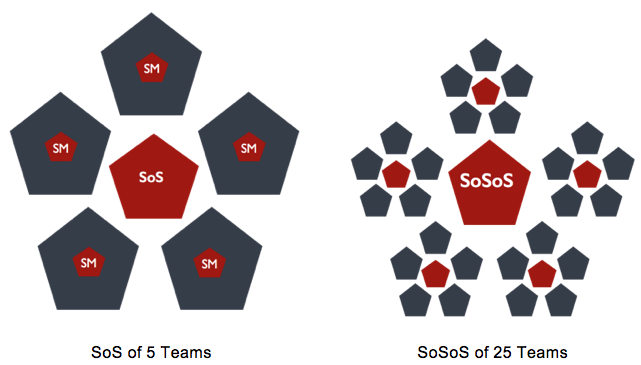
\includegraphics[width=1.0\linewidth]{Sos-R2.png}

\textbf{\textsc{note:}} Podczas gdy Przewodnik po Scrumie definiuje optymalny rozmiar jako 3 do 9 osób, badanie Harvardu ustaliło optymalny rozmiar zespołu jako 4.6 osoby.\footnote{Hackman, J Richard, Leading teams: Setting the stage for great performances, Harvard Business Press, 2002} Eksperymenty z wysoce wydajnymi Zespołami Scrumowymi powtarzalnie pokazały, że 4 lub 5 osób wykonujących pracę jest optymalnym rozmiarem. Kluczowe dla liniowej skalowalności jest stosowanie tego wzorca w odniesieniu do liczby zespołów w SoS. Dlatego, w diagramach powyżej i poniżej pięciokąty zostały wybrane jako reprezentacja zespołu 5 osób. Te diagramy maja służyć wyłącznie jako przykład, a diagram twojej organizacji może znacznie się różnić.

\subsection{Skalowanie Product Owner Team}

Tak samo jak SoSy mogą rosnąć do SoSoSów, zespoły Product Owner Team mogą rozszerzać się korzystając z tego samego mechanizmu. Nie ma konkretnej nazwy na te rozszerzone jednostki ani ich CPO nie mają konkretnej nazwy. Zachęcamy każdą organizację stworzyć własne nazwy. Na poniższych diagramach wybraliśmy dodanie "Chief" do tytułu tych PO, żeby się wyróżniali.

Przykładowe diagramy:

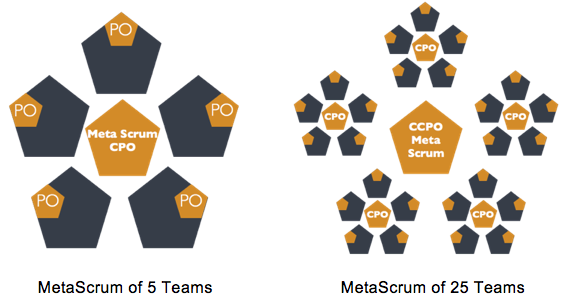
\includegraphics[width=1.0\linewidth]{MetaScrum-R2.png}

\textbf{UWAGA:} Jak wspomniano powyżej, pięciokąty reprezentują idealnej wielkości Zespoły Scrumowe i idealnej wielkości zespoły Product Owner Team.Te diagramy mają służyć wyłącznie jako przykład, a diagram twojej organizacji może znacznie się różnić.

\section{Cykl Scrum Mastera Cycle - Koordynacja "Jak"}

Organizacja SM (SM, SoSM, EAT) pracują jako całość, żeby uzupełnić komponenty Cyklu Scrum Mastera. Komponentami unikalnymi dla Cyklu Scrum Mastera są: \textbf{Ciągłe Ulepszanie i Usuwanie Przeszkód, Międzyzespołowa Koordynacja oraz Wdrażanie}.
%deploymnet - wdrożenie
%release - wydanie
\subsection{Ciągłe Ulepszanie i Usuwanie Przeszkód}

Celami Ciagłego Usprawniania i Usuwania Przeszkód są:

\begin{itemize}
	\item identyfikacja przeszkód i przeramowanie ich w okazje.
	\item utrzymanie zdrowego i ustrukturyzowanego środowiska dla priorytetyzacji i usuwania przeszkód, a następnie weryfikacja wynikających usprawnień.
	\item zapewnienie widoczności w organizacji, żeby umożliwić zmianę.
\end{itemize}

\subsection{Międzyzespołowa Koordynacja}

Celami Międzyzespołowej Koordynacji są:

\begin{itemize}
	\item skoordynować podobne procesy pomiędzy wieloma powiązanymi zespołami.
	\item złagodzić wpływ międzyzespołowych zależności, żeby zapewnić, że nie staną się przeszkodami.
	\item utrzymać uzgodnienie zasad zespołowych i wytycznych dla spójnego wytwarzania.
\end{itemize}

\subsection{Wdrażanie}

Ponieważ celem SoS jest funkcjonować jako zespół wydaniowy, wdrażanie produktu leży w ich zakresie, podczas gdy co wydanie zawiera leży w zakresie Product Ownerów. Zatem, celami Wdrażania są:

%Product Owners - tłumaczyć czy nie

\begin{itemize}
	\item dostarczyć stały przepływ wartościowego, skończonego produktu do klientów.
	\item zintegrować pracę różnych zespołów w jeden spójny produkt.
	\item zapewnić wysoką jakość doświadczania klienta.
\end{itemize}

\section{Cykl Product Ownera - Koordynowanie "Co"}

Organizacja PO (Product Owner, CPO, Executive MetaScrum) pracują jako całość, żeby uzupełnić komponenty Cyklu Product Ownera. Komponentami unikalnymi dla Cyklu Product Ownera są: \textbf{Strategiczna Wizja, Priorytetyzacja Backlogu, Dekompozycja i Pielęgnacja Backlogu oraz Planowanie Wydań}.

\subsection{Strategiczna Wizja}

Celami Strategicznej Wizji są:

\begin{itemize}
	\item jasno zorientować całą organizację wzdłuż wspólnej drogi na przód.
	\item przekonująco wyrazić dlaczego organizacja istnieje.
	\item opisać co organizacja zrobi, żeby wykorzystać kluczowe aktywa do wsparcia jej misji.
	\item odpowiedzieć na dynamicznie zmieniające się warunki na rynku..
\end{itemize}

\subsection{Priorytetyzacja Backlogu}

Celami Priorytetyzacji Backlogu są:

\begin{itemize}
	\item zidentyfikować jasny porządek produktów, funkcjonalności i usług do dostarczenia.
	\item odzwierciedlić tworzenie wartości, mitygację ryzyka i wewnętrzne zależności w porządku na backlogu.
	\item spriorytetyzować wysokopoziomowe inicjatywy w całej zwinnej organizacji przed Dekompozycją Backlogu i Pielęgnacją.
\end{itemize}

\subsection{Dekompozycja i Pielęgnacja Backlogu}

Celami Dekompozycji i Pielęgnacji Backlogu są:

\begin{itemize}
	\item rozbić złożone produkty i projekty w niezależne, funkcjonalne elementy, które mogą być ukończone przez jeden zespół w jednym Sprincie.
	\item zebrać i wydobyć istotę wyłaniających się wymagań i informacji zwrotnej od klienta.
	\item zapewnić, że wszystkie elementy backlogu są naprawdę "Gotowe", żeby mogły być pobrane przez poszczególne zespoły.
\end{itemize}

\subsection{Planowanie Wydań}

Celami Planowania Wydań są:

\begin{itemize}
	\item prognozować wdrożenie kluczowych funkcjonalności i zdolności.
	\item komunikować oczekiwania co do wdrożeń interesariuszom.
	\item aktualizować priorytetyzację, jeśli potrzeba.
\end{itemize}

Zauważ, że Planowanie Wydań może dotyczyć jednego lub wielu wydań produktu do klienta. Jest to horyzont planowania wyższego poziomu niż jeden Sprint, zazwyczaj pokrywające okres od 1 do 6 miesięcy.

\section{Łączenie Cykli PO/SM}

Cykle PO i SM Cycles mają dwa punkty styku: \textbf{Proces Poziomu Zespołu and Feedback dla Produktu i Wydania}. Oba cykle potrzebują  \textbf{Metryk i Przejrzystości}.

\subsection{Proces Poziomu Zespołu}

\textbf{Proces Poziomu Zespołu} stanowi pierwszy punkt styku pomiędzy Cyklami Scrum Mastera i Product Ownera i jest jasno wyłożony w Przewodniku po Scrumie. Składa się z trzech artefaktów, pięciu wydarzeń i trzech ról. Celami Procesu Poziomu Zespołu są:

\begin{itemize}
	\item zmaksymalizować przepływ ukończonej i przetestowanej pracy.
	\item z czasem zwiększyć wydajność zespołu.
	\item działać w sposób, który jest utrzymywalny i wzbogacający dla zespołu.
	\item przyspieszyć pętlę feedbacku od klienta.
\end{itemize}

\subsection{Feedback dla Produktu i Wydania}

Komponent \textbf{Feedback dla Produktu i Wydania} jest drugim punktem, w którym stykają się Cykle PO i SM. Feedback dla produktu napędza ciągłe ulepszanie poprzez dostosowywanie Product Backlogu, podczas gdy feedback dla Wydania napędza ciągłe ulepszanie poprzez dostosowywanie mechanizmu Wdrażania. Celami pozyskiwania i analizowania feedbacku są:

\begin{itemize}
	\item sprawdzić nasze założenia.
	\item zrozumieć jak klienci korzystają z produktu i wchodzą z nim w interakcję.
	\item uchwycić pomysły na nowe funkcjonalności i funkcje.
	\item zdefiniować ulepszenia w istniejącej funkcjonalności.
	\item zaktualizować postęp względem ukończenia produktu/projektu, żeby dopracować planowanie wydań i uzgodnienie z interesariuszami.
	\item zidentyfikować ulepszenia w metodach i mechanizmach wdrażania.
\end{itemize}

\subsection{Metryki i Przejrzystość}

Radykalna przejrzystość jest kluczowa w Scrum do optymalnego funkcjonowania, ale jest możliwa jedynie wtedy, kiedy organizacja przyjęła wartości Scruma. To daje organizacji możliwość uczciwego określenia postępu oraz sprawdzania i dostosowywania jej produktów i procesów. To jest podstawa empirycznej natury Scruma jak to zostało wyłożone w Przewodniku po Scrumie.

Oba Cykle SM i PO wymagają metryk, na podstawie których będą podejmowane decyzje w oddzielnych organizacjach SM i PO. Metryki mogą być unikalne dla każdej z organizacji jak i dla poszczególnych funkcji w tych organizacjach. Scrum@Scale nie wymaga żadnego konkretnego zestawu metryk, ale sugeruje, że absolutne minimum tego, co organizacja powinna mierzyć:

\begin{itemize}
	\item Produktywność - n.p. zmiana w ilości Działającego Produktu dostarczana na Sprint
	\item Dostarczanie Wartości - n.p. wartość biznesowa na jednostkę wysiłku zespołu
	\item Jakość - n.p. wskaźnik błędów lub przestój usługi
	\item Utrzymywalność - n.p. zadowolenie zespołu
\end{itemize}

Celami posiadania Metryk i Przejrzystości są:

\begin{itemize}
	\item dostarczenie wszystkim osobom podejmującym decyzje, włączając w to członków zespołów, odpowiedniego kontekstu do podejmowania dobry decyzji.
	\item skrócenie cyklu feedbacku na ile to możliwe, żeby uniknąć nadmiernej korekty.
	\item wymaganie minimalnego dodatkowego wysiłku ze strony zespołów, interesariuszy lub liderów.
\end{itemize}

\section{Jak zacząć ze Scrum@Scale}

Podczas implementacji rozległej sieci zespołów, kluczowe jest zbudowanie skalowalnego \textbf{Modelu Referencyjnego} dla małego zestawu zespołów. 
Jakiekolwiek niedociągnięcia w implementacji Scruma będą powiększone, kiedy zostanie wdrożone wiele zespołów. Wiele z początkowych problemów skalowania będzie się zasadami organizacji i procedurami lub praktykami deweloperskimi, które blokują wydajność i frustrują zespoły.

Dlatego, pierwszym wyzwaniem jest stworzyć mały zestaw zespołów, który dobrze implementuje Scruma. Najlepszym sposobem do osiągnięcia tego jest stworzenie \textbf{Executive Action Team (EAT)}, który jest odpowiedzialny za rozwój i wykonanie strategii transformacji. EAT musi składać się z osób, które są politycznie i finansowo umocowane do tego, żeby zapewnić istnienie Modelu Referencyjnego. Ten zbiór zespołów przepracowuje zagadnienia organizacyjne, które blokują zwinność i tworzy Model Referencyjny dla Scruma, który jest sprawdzony w organizacji i może być użyty jako wzorzec dla skalowania Scruma w całej organizacji.

W miarę jak powiększa się Model Referencyjny, przeszkody i wąskie gardła, które opóźniają dostarczanie, produkują marnotrawstwo albo zagrażają zwinności biznesowej stają się oczywiste. Najbardziej efektywnym sposobem na eliminowanie tych problemów jest rozszerzenie Scruma w organizacji tak, żeby cały strumień dostarczania wartości był zoptymalizowany.

Scrum@Scale osiąga liniową skalowalność w produktywności przez nasycenie organizacji Scrumem i organiczne dystrybuowanie prędkości i jakości w sposób spójny z unikalną strategią, produktami i usługami organizacji.

\section{Kilka Uwag o Projektowaniu Organizacji}

Bezskalowa natura Scrum@Scale pozwala na oparcie projektu organizacji na komponentach tak jak framework sam w sobie. To pozwala na balansowanie i refaktoryzację zespołów w odpowiedzi na rynek. W miarę jak organizacja rośnie, może okazać się ważne opanowanie korzyści płynących z rozproszonych zespołów. Niektóre organizacje sięgają po talenty nie dostępne w inny sposób i są zdolne do rozszerzania się i kurczenia wedle potrze poprzez outsourcing. Scrum@Scale pokazuje jak to zrobić unikając długich czasów opóźnienia, problemów z komunikacją i podrzędnej jakości, umożliwiając liniową skalowalność zarówno w rozmiarze jak i globalnym rozproszeniu.\footnote{Sutherland, Jeff and Schoonheim, Guido and Rustenburg, Eelco and Rijk, Maurits, "Fully distributed scrum: The secret sauce for hyperproductive offshored development teams", AGILE'08. Conference, IEEE: 339-344, 2008}

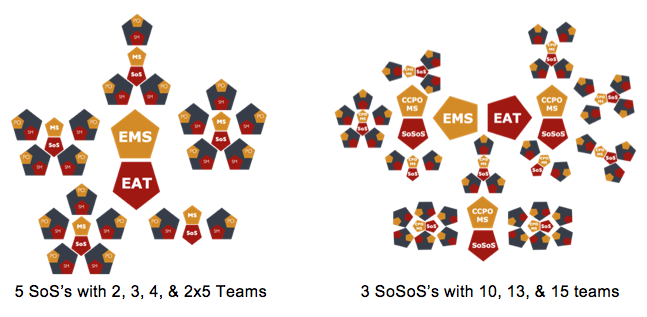
\includegraphics[width=1.0\linewidth]{VariableSoS-R2.png}
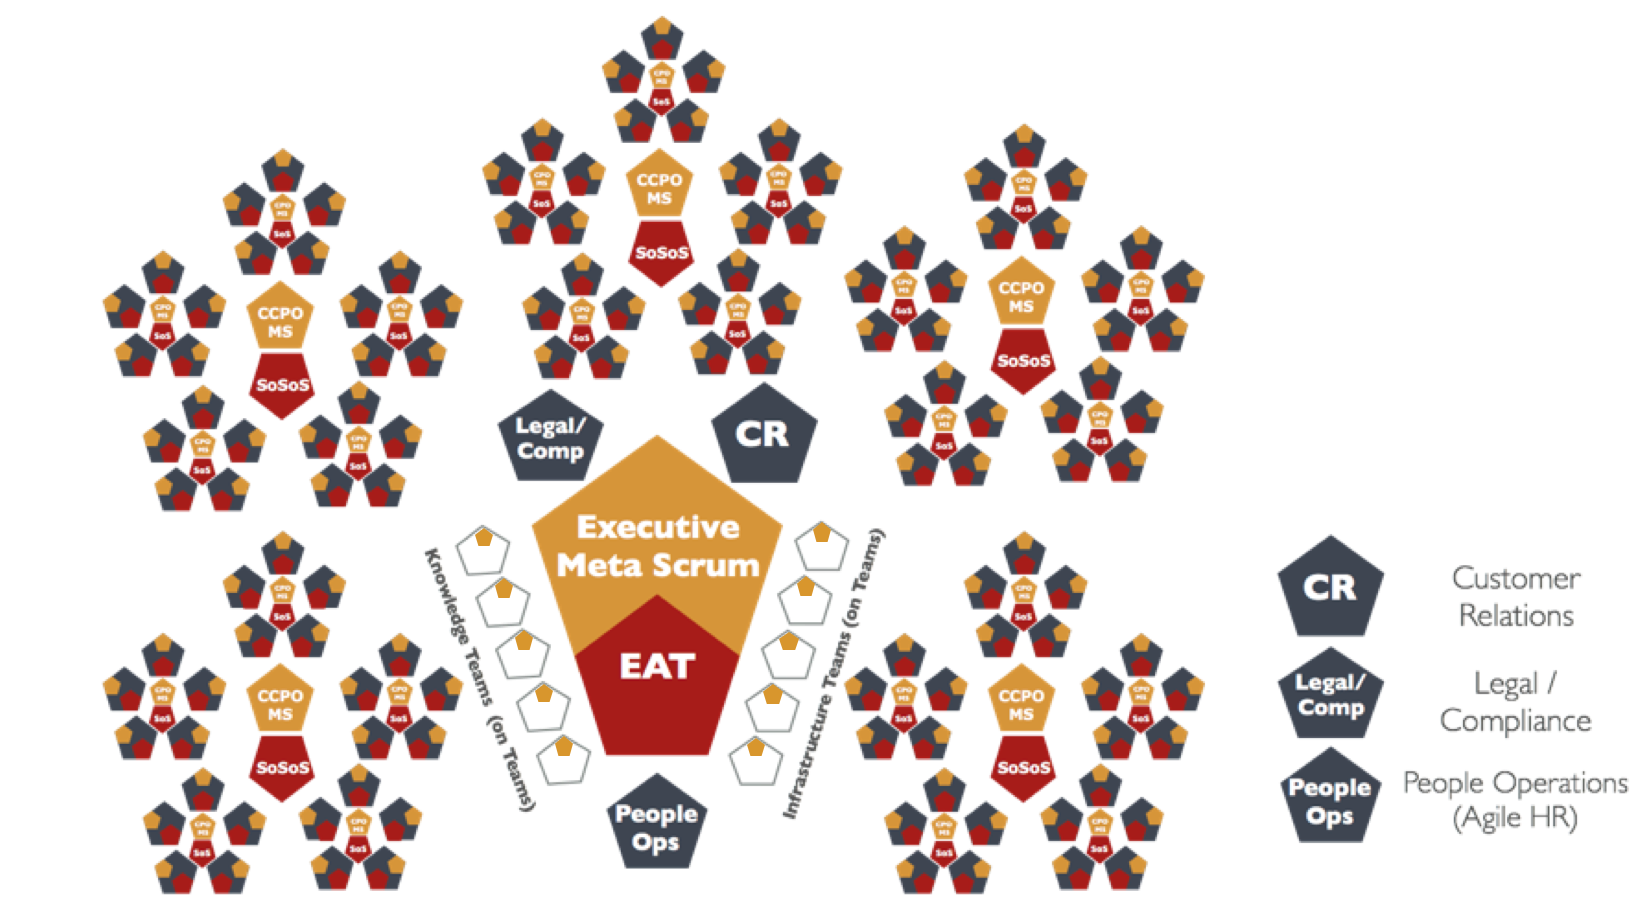
\includegraphics[width=1.0\linewidth]{OrganizationalDiagram.png}

	Na tym diagramie organizacyjnym \textbf{Zespoły Knowledge \& Infrastructure Team} reprezentują wirtualne zespoły specjalistów, których jest zbyt mało, żeby wchodzić w skład każdego zespołu. Koordynują się z Zespołami Scrumowymi jako grupa poprzez kontrakty poziomie usług gdzie zgłoszenia dla każdej specjalizacji przepływają przez PO, który zamienia je w przejrzysty, uporządkowany backlog. Ważna uwaga, te zespoły NIE są silosami osób, które siedzą razem (dlatego są oni reprezentowani jako niewypełnione pięciokąty); ich członkowie zespołów znajdują się w konkretnych Zespołach Scrumowych, tworzą swój własny wirtualny Scrum w celu dystrybuowania backlogu i ulepszania procesu.

\textbf{Customer Relations, Legal / Compliance i People Operations} są tutaj ujęte ponieważ są niezbędnymi częściami organizacji i będą istniały jako samodzielne, niezależne Zespoły Scrumowe, od których mogą zależeć wszystkie pozostałe. 

Ostatnia uwaga na temat reprezentowania EAT i EMS: na tym diagramie są pokazane jako nachodzące na siebie, ponieważ niektórzy członkowie znajdują się w obu tych zespołach. W bardzo małych organizacjach lub implementacjach, EAT i EMS mogą całkowicie składać się z tych samych członków zespołu.

\section{Przypis Końcowy}

Scrum@Scale jest zaprojektowany do skalowania produktywności, doprowadzając całą organizację do dostarczania dwa razy więcej dwa razy szybciej z wyższą jakością i w znacznie ulepszonym środowisku pracy. Wielkie organizacje, które prawidłowo zaimplementują ten framework mogą obniżyć koszt swoich produktów i usług równocześnie podnosząc jakość i innowację.

Scrum@Scale jest zaprojektowany to do nasycenia organizacji Scrumem. Wszystkie zespoły, włączając Kierownictwo, Zasoby Ludzkie, Prawny, Doradztwo i Szkolenia oraz zespoły produktowe i usługowe implementują ten sam styl Scruma  usprawniając i wzmacniając organizację.

Dobrze zaimplementowany Scrum może zarządzać całą organizacją.

\section{Podziękowania}

Dziękujemy IDX ze stworzenie Scrum of Scrums, który po raz pierwszy pozwolił zeskalować Scrum na setki zespołów,\footnote{Sutherland, Jeff, "Inventing and Reinventing SCRUM in five Companies", Sur le site officiel de l'alliance agile, 2001} PatientKeeper za stworzenie MetaScrum,\footnote{Sutherland, Jeff, "Future of scrum: Parallel pipelining of sprints in complex projects", Proceedings of the Agile Development Conference,  IEEE Computer Society 90-102,  2005.} który umożliwił błyskawiczne wdrożenie innowacyjnego produktu i OpenView Venture Partners za skalowanie Scruma do całej organizacji. \footnote{Sutherland, Jeff and Altman, Igor, "Take no prisoners: How a venture capital group does scrum", Agile Conference, 2009. AGILE'09, IEEE 350-355.  2009} Doceniamy wsad od Intel, gdzie ponad 25,000 ludzi robi Scrum, który nauczył nas, że "nic się nie skaluje" poza bezskalową architekturą i SAP z największą organizacją produktową Zespołów Scrumowych, który nas nauczył, że zaangażowanie kierownictwa jest kluczowe, żeby 2000 Zespołów Scrumowych pracowało razem.

Agile coache'e i trenerzy implementujący te koncepcje w Amazon, GE, 3M, Toyota, Spotify, Maersk, Comcast, AT\&T i wielu innych firmach pracując z Jeffem Sutherlandem byli pomocni w testowaniu tych koncepcji poprzez szeroki wachlarz firm i różnych domen.

W końcu, Avi Schneier, Alex Sutherland i Jessica Larsen byli nieocenieni w formułowaniu i edytowaniu tego dokumentu.

Dziękuję Markowi Hańskiemu za feedback i pracę edytorską w polskiej edycji dokumentu.

\pagebreak

\printbibliography

\end{document}
